\qrchapter{https://forgottenpillar.com/rsc/en-fp-chapter2}{The Fundamental Principles}

\qrchapter{https://forgottenpillar.com/rsc/en-fp-chapter2}{Kanuni za Msingi}

Suala halisi kwa mujibu wa sura ya kumi ya Shuhuda Maalum ni kuhusu kuenda kinyume na msingi wa imani yetu, ambao ulianzishwa mwanzoni mwa kazi yetu.

\egw{\textbf{Msingi huu ulijengwa na Mfanyakazi Mkuu}, na \underline{kuhimili} dhoruba na tufani. Je, watamruhusu mtu huyu \textbf{kuwasilisha mafundisho yanayopinga uzoefu wa awali} wa watu wa Mungu? Wakati umefika wa kuchukua hatua maalum.}[SpTB02 54.2; 1904][https://egwwritings.org/read?panels=p417.276]

Kellogg aliwasilisha mafundisho ambayo yanakataa uzoefu uliopita. Katika sehemu nyingine, aliandika kuhusu Kellogg:

\egw{Nina wasiwasi sana kuhusu Dkt. Kellogg. Katika mambo mengi, kozi yake haipendezi Bwana. Inaonekana kuwa \textbf{ni rahisi sana kwake kuachana na \underline{kanuni za msingi}}. Yuko katika hatari kubwa \textbf{ya kutoshikilia imani yake ya mwanzo kwa thabiti } hadi mwisho.}[Lt138-1902.5; 1902][https://egwwritings.org/read?panels=p9219.11]

Tatizo lilikuwa ni kujitenga na kanuni za msingi—lakini si watu wote walitambua hiyo. Hasa watu wakuu na maarufu katika kazi; walisahau jinsi Bwana alivyowaongoza na mafundisho Yake ya awali.

\egw{Nimekuwa nikitumaini kwamba kungekuwa na mageuzi ya kina, na kwamba \textbf{kanuni} ambazo tulizipigania \textbf{siku za kwanza}, na ambazo zilitolewa katika nguvu ya Roho Mtakatifu, \textbf{zingedumishwa}.}[SpTB02 56.3; 1904][https://egwwritings.org/read?panels=p417.287]

Ni kanuni gani tulizopigania katika siku za kwanza? Ni upi msingi wa imani yetu?

\egw{Kama watu maalum, tunapaswa \textbf{kusimama kidete kwenye jukwaa la ukweli wa milele} ambao umestahimili mtihani na majaribio. Tunapaswa \textbf{kushikilia nguzo za hakika za imani yetu}. \textbf{\underline{Kanuni za ukweli}} ambazo Mungu ametufunulia \textbf{ndio msingi wetu wa kweli}. Zimetufanya tulivyo...}[SpTB02 51.2; 1904][https://egwwritings.org/read?panels=p417.261]

\egwinline{Kanuni za ukweli} ambazo Mungu amefunua \egwinline{ndio msingi wetu wa kweli}. Anaziita kanuni hizi jukwaa la ukweli wa milele. Anarejelea kanuni hizi kama \egwinline{nguzo kamili za imani yetu}[SpTB02 51.2; 1904][https://egwwritings.org/read?panels=p417.261].

Anakumbuka uzoefu uliopita wa wazee wetu, kama James White, Joseph Bates, Mzee Edson, baba Pierce, jinsi Mungu alivyofanya kazi nao mpaka \egwinline{pointi kwa pointi}, \egwinline{\textbf{pointi kuu za imani yetu} zikawekwa wazi}. Alikumbuka jinsi \egwinline{msingi huu ulijengwa na Mjenzi mkuu,} na kuhakikishia kwamba \egwinline{utahimili dhoruba na tufani}. Kwa kumalizia, anatuthibitishia mapenzi ya Mungu kwetu kuhusu kanuni hizi. Mungu \egwinline{anatuita \textbf{tushike imara}, kwa mshiko wa imani, \textbf{kanuni za msingi ambazo mamlaka wake ni usio na shaka}}.

Tunaona semi kadhaa ambazo Dada White alitumia kwa msingi wa imani yetu: “\textit{jukwaa la ukweli wa milele},” “\textit{nguzo za imani yetu},” “\textit{kanuni za ukweli},” “\textit{pointi kuu},” “\textit{alama za njia},” “\textit{kanuni za msingi},” na “\textit{kanuni za kimsingi}”. Semi hizi zinaashiria jambo moja—msingi wa imani yetu. Leo tunaposikia semi hizi, kwa namna fulani hazifikishi habari yoyote thabiti. Lakini kwa Waadventista Wasabato wa siku za Ellen White, semi hizi zilikuwa na maana ya wazi sana. Semi hizi zote zinaashiria muhtasari wa umma wa imani ya Waadventista Wasabato iitwayo \emcap{Kanuni za Msingi}, kama ilivyoelezwa zaidi hapa chini.

Mungu \egwinline{anatuita \textbf{kushika kwa uthabiti}, kwa mshiko wa imani, \textbf{\underline{kanuni za msingi}} ambazo zinatokana na \textbf{mamlaka isiyotiliwa shaka}.} Hii ni rejeo kwa mambo makuu ya imani ya Waadventista Wasabato ambayo Mungu aliwafunulia wazee wa Waadventista \egwinline{baada ya kupita kwa wakati wa 1844,} wakati kundi la watu wenye bidii, waungwana na wa kweli \egwinline{walitafuta ukweli kama hazina iliyofichwa.} Huu ulikuwa \textit{msingi wa imani yetu}. Wazee wetu walianzisha rasmi Kanisa la Waadventista Wasabato mwaka 1863, na walifundisha kweli hizi walizoziita “\textit{kanuni za msingi}.” Lakini mara nyingi, Waadventista Wasabato waliwasilishwa vibaya hadharani. Kwa sababu hii, mwaka 1872, wazee wetu walichapisha waraka ulioitwa “\textit{A Declaration of the Fundamental Principles, Taught and Practiced by the Seventh-day Adventists}” ili kutangaza hadharani, kwa ufupi, ni \emcap{kanuni za msingi} gani Waadventista Wasabato walifundisha na kutenda. Hizi \emcap{Kanuni za Msingi} zilichapishwa mara kwa mara kama kijitabu, zilikuwepo katika magazeti yetu, na zilichapishwa kila mwaka katika Vitabu vya Mwaka vya Waadventista katika maisha yote ya Ellen White.\footnote{Tazama \hyperref[appendix:timeline]{Kanuni za Msingi - Mfululizo wa matukio} kwa maelezo zaidi.} Kwa hiyo, Ellen White aliporejea “\textit{kanuni za msingi},” hii haikuwa kauli isiyoeleweka au isiyowazi, kwani kanisa la Waadventista Wasabato lilikuwa limetangaza rasmi na hadharani ni \emcap{kanuni za msingi} gani. Katika utangulizi wa waraka huu, tunasoma lengo la waraka huu.

\begin{figure}
    \centering
    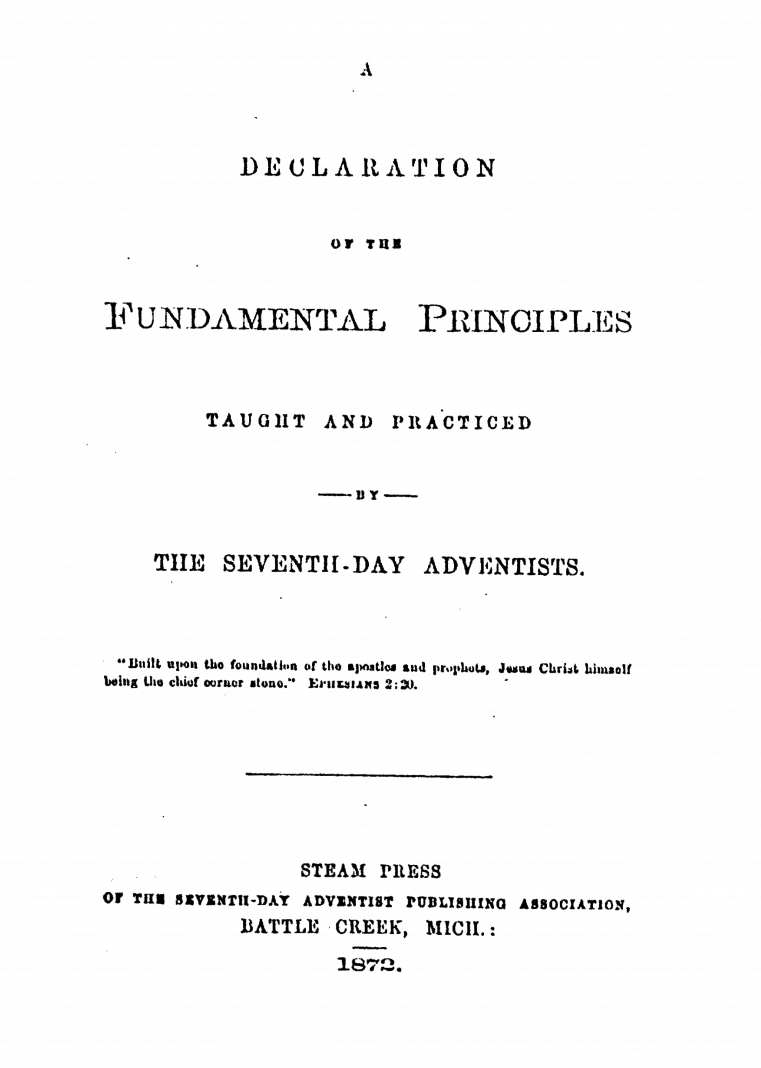
\includegraphics[width=1\linewidth]{images/declaration-of-the-fundamental-principles.PNG}
    \caption*{Scan of the Declaration of the Fundamental Principles, 1872.}
    \label{fig:declaration-of-the-fundamental-principles}
\end{figure}

\begin{figure}
    \centering
    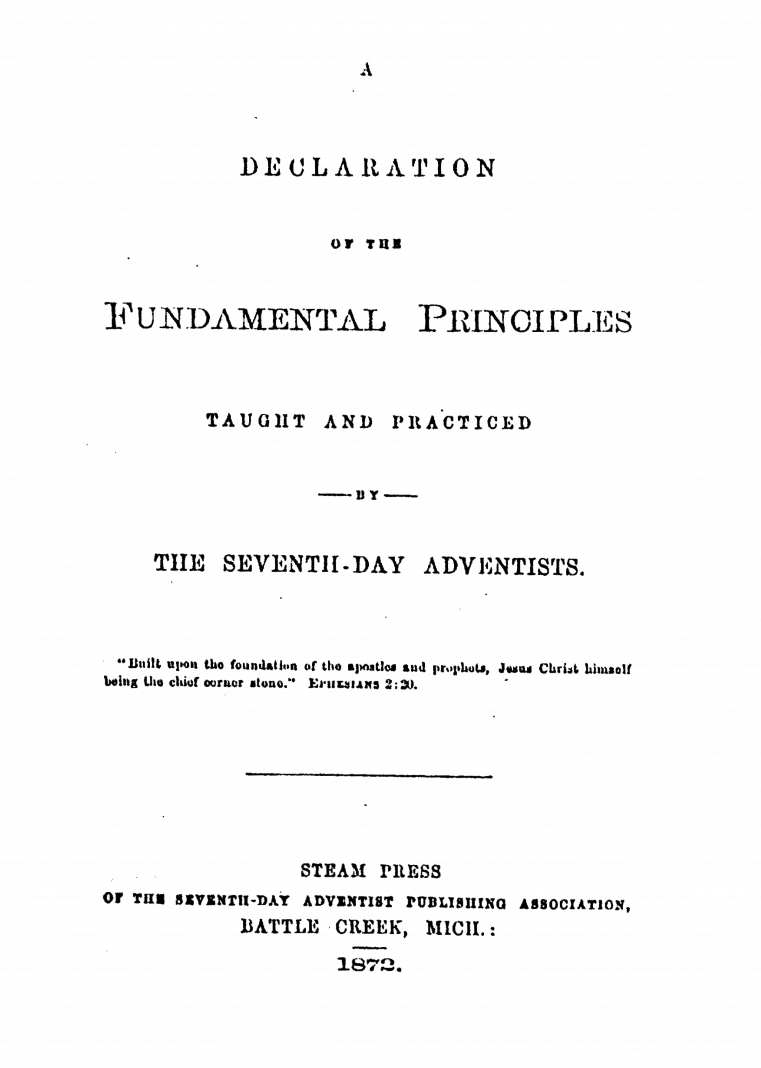
\includegraphics[width=1\linewidth]{images/declaration-of-the-fundamental-principles.PNG}
    \caption*{Picha ya Tamko la Kanuni za Msingi, 1872.}
    \label{fig:declaration-of-the-fundamental-principles}
\end{figure}

\others{Katika kuwasilisha kwa \textbf{umma} muhtasari huu wa imani yetu, tunataka ieleweke kwa uwazi kwamba \textbf{hatuna vifungu vya imani, kanuni za imani, au nidhamu, }\textbf{\underline{kando na Biblia}}. \textbf{Hatuweki} haya kuwa na \textbf{mamlaka yoyote juu ya watu wetu}, \textbf{wala hayakusudiwi kufanya usawa kati yao}, \textbf{kama mfumo wa imani}, \textbf{bali ni taarifa fupi ya \underline{wanayoamini kwa umoja mkubwa}}. Mara nyingi tunaona umuhimu wa kukutana na maswali juu ya mada hii, na wakati mwingine kusahihisha taarifa za uwongo zinazosambazwa dhidi yetu, na kuondoa hisia potofu wanazo wale ambao hawajapata nafasi ya kufahamiana na imani na utendaji wetu. Lengo letu la pekee ni kukutana na haya.}

\othersnogap{\textbf{Kama Waadventista Wasabato tunatamani tu kwamba msimamo wetu utaeleweka}; na tunatamani sana hili kwa sababu wapo wengi wanaojiita Waadventista bali wanashikilia maoni ambayo hatuwezi kuwa na huruma nayo, ambayo baadhi yake, tunafikiri, yanapindua kanuni zilizo wazi na muhimu zaidi zilizowekwa wazi katika neno la Mungu...}[The Fundamental Principles 1872, p. 3.1][https://egwwritings.org/read?panels=p928.8]

Muhtasari huu wa imani ulikuwa na Pointi 25, ambayo yaliwakilisha \others{wanayoamini kwa umoja mkubwa} Waadventista Wasabato. Mambo haya 25 yalijumuisha \egwinline{\textbf{msingi} ambao \textbf{uliwekwa mwanzoni} mwa kazi yetu \textbf{kwa kujifunza neno kwa maombi} na kwa ufunuo}. Mnamo 1904, Dada White alituambia kwamba \egwinline{juu ya \textbf{msingi huu} tumekuwa tukijenga kwa \textbf{miaka hamsini iliyopita}.} Hizi ndizo \egwinline{\textbf{kanuni za kimsingi ambazo msingi wake ni mamlaka isiyotiliwa shaka}}, kwamba Mungu \egwinline{anatuita \textbf{tushike kwa uthabiti}, pamoja na mshiko wa imani}. Kwa maneno mengine, alirudia, \egwinline{tunapaswa \textbf{kushikilia nguzo za hakika za imani yetu}}.

Mnamo 1904, Dada White aliandika kuhusu \egwinline{\textbf{juhudi za adui kudhoofisha msingi wa imani yetu}}. Aliandika kuhusu vuguvugu ambalo \egwinline{lingehusisha \textbf{kuacha} mafundisho ambayo yanasimama kama \textbf{nguzo za imani yetu}}. Matengenezo haya yakikubaliwa yangetupilia mbali \egwinline{\textbf{kanuni za ukweli} ambazo Mungu katika hekima yake amefunulia kanisa la masalio} na \egwinline{\textbf{kanuni za kimsingi} ambazo zimedumisha kazi hiyo kwa miaka hamsini iliyopita \textbf{zingehesabiwa kuwa makosa}.} Vuguvugu hili lilianza wakati ambapo Dk. John H. Kellogg alichapisha kitabu, “Hekalu Hai”.

\egw{Takriban wakati ambapo ‘Hekalu Hai’ ilichapishwa, ilipita mbele yangu katika msimu wa usiku, \textbf{maono zilizoonyesha kwamba hatari fulani ilikuwa inakaribia}, na hivyo ni lazima nijitayarishe kwa \textbf{kuandika mambo} ambayo Mungu amenifunulia \textbf{kuhusu \underline{kanuni za msingi wa imani yetu}}.}[SpTB02 52.3; 1904][https://egwwritings.org/read?panels=p417.267]

Kwa kuchapisha “Hekalu Hai”, \textbf{kanuni za msingi wa imani yetu} \textbf{zingedhoofishwa} \egwinline{kupitia uenezaji wa \textbf{nadharia potofu}} zilizomo humo.

\egw{Nimeagizwa na mjumbe wa mbinguni kwamba baadhi ya hoja katika kitabu, ‘Living Temple,’ hazifai na kwamba \textbf{hoja hizi zitapotosha} akili za wale ambao hawajasimama kikamilifu juu ya \textbf{kanuni za msingi} za ukweli wa sasa. Inatanguliza yale ambayo si chochote bali dhana tu kuhusiana na \textbf{\underline{umbile la Mungu na mahali uwepo Wake ulipo}}.}[SpTB02 51.3; 1904][https://egwwritings.org/read?panels=p417.262]

Dada White anakazia sana kuonyesha kwamba hoja iliyo katika kitabu cha Living Temple,\egwinline{\textbf{zitapotosha}} kutoka kwa\egwinline{\textbf{kanuni za msingi} za ukweli wa sasa}. Hoja hizi ni kuhusiana na\egwinline{\textbf{umbile la Mungu na mahali uwepo Wake upo}}.

Kama ilivyoelezwa hapo awali, neno ‘\textit{personality}’, katika muktadha wa karne ya kumi na tisa, inamaanisha “\textit{ubora au hali ya kuwa Nafsi}”\footnote{\href{https://www.merriam-webster.com/dictionary/personality}{Merriam-Webster Dictionary}, neno ‘\textit{personality}’}. Kwa maneno mengine, neno hili huwasilisha jibu kwa swali, “\textit{ni nini kinachofafanua yeyote yule kuwa Nafsi?}”, “\textit{Ni nini ubora au hali ya Nafsi kuwa Nafsi?}” Katika suala la \emcap{umbile la Mungu}, swali ni, “\textit{Je, Mungu ni Nafsi na ni nini kinachomfafanua kuwa Nafsi? Ni nini ubora au hali ya Mungu kuwa Nafsi?}”

Hoja ya Dkt. Kellogg kuhusu maswali hayo iliyoonyeshwa katika kitabu Living Temple, ni\egwinline{halifu}. Maoni, kuhusu\egwinline{\textbf{umbile la Mungu na mahali uwepo Wake ulipo}},\egwinline{yanayotetewa katika kitabu, hayana idhini ya Mungu, na ni \textbf{mtego ambao adui alikuwa ametayarisha kwa siku za mwisho}}. Kama tunaishi katika siku za mwisho, tunapaswa kujiuliza maswali haya. Vivyo hivyo, tunapaswa kuhoji uhalali wa kibiblia wa kauli zilizo katika \emcap{Kanuni za Msingi} kuhusu \emcap{umbile la Mungu} na mahali uwepo wake ulipo. Je, \emcap{Kanuni za Msingi} zinafafanuaje Mungu kuwa Nafsi, na zinasema nini kuhusu uwepo wake?

Jambo la kwanza lililoorodheshwa hapa chini linahusu \emcap{umbile la Mungu} na uwepo wake. La pili linatoa muktadha wa la kwanza. Tafadhali zingatia maswali haya unapoyasoma: Nani anaashiriwa kuwa Mungu mmoja? Mungu anafafanuliwaje kuwa Nafsi au kwa maneno mengine, ni nini ubora au hali ya Yeye kuwa Nafsi? Je, mambo haya yanazungumziaje uwepo wa Mungu?

\others{“I – Kwamba kuna \textbf{Mungu mmoja}, \textbf{\underline{nafsi wa kibinafsi, wa kiroho}}, \textbf{Muumba wa vitu vyote}, mwenye uwezo wote, mwenye kujua yote, na wa milele, asiye na kikomo katika hekima, utakatifu, haki, wema, ukweli, na rehema; asiyebadilika, na \textbf{\underline{aliye kila mahali kupitia kwa mwakilishi wake, Roho Mtakatifu}}. Zab. 139:7.”}

\othersnogap{II – Kwamba kuna \textbf{Bwana mmoja Yesu Kristo, }\textbf{\underline{Mwana wa Baba wa Milele}}, ambaye \textbf{\underline{kupitia}}\textbf{ kwake Mungu aliumba vitu vyote}, na kupitia kwake vitu hivyo vinadumu; …“}[The Fundamental Principles 1889, point no. 1.,2.,.] \footnote{Tazama \hyperref[chap:appendix]{Kiambatisho} kwa orodha kamili ya Kanuni za Msingi} \footnote{Kutoka 1872 hadi 1914, Kanuni za Msingi zilisalia thabiti na bila mabadiliko, isipokuwa mwaka 1889, wakati Uriah Smith alipoongeza pointi tatu mpya. Lakini katika miaka yote hiyo, pointi zinazohusiana na “\textit{umbile la Mungu}” na “\textit{mahali uwepo Wake upo}” zilisalia sawa.}

Katika wakati wa Ellen White, Waadventista Wasabato waliamini katika Mungu mmoja—nafsi wa kibinafsi, wa kiroho, Muumba wa vitu vyote—na waliamini kwamba Mungu huyu aliumba kila kitu kupitia kwa Mwana wake Yesu Kristo. Walimwita Baba, Mungu mmoja, na walimwita Kristo, Mwana wa Mungu. Ubora au hali ya Mungu kuwa Nafsi inaonyeshwa katika neno “\textit{nafsi ya kibinafsi, ya kiroho}”. Kuhusu uwepo wake, \emcap{Kanuni za Msingi} zinaeleza kuwa yuko kila mahali kupitia kwa mwakilishi wake, Roho Mtakatifu. Maana ya kanuni hizi inahitaji umakini maalum sana. Hii itakuwa mada ya masomo yetu yafuatayo.

\section*{Mtihani}

Ni wazi kuwa \emcap{kanuni hizi za msingi} hazina fundisho la Utatu! Kwa usahihi zaidi, maoni “\textit{watatu katika mmoja},” au “\textit{mmoja katika watatu}”, kuhusiana na Mungu, hayapatikani popote—ambayo yapo katika \textit{Imani za Msingi} za leo. Baba pekee ndiye anayetajwa kama “\textit{Mungu mmoja}”. Lakini kabla ya kuhitimisha haraka, na kushutumu fundisho la Utatu kama\egwinline{\textbf{nadharia za uwongo,}} ambazo\egwinline{\textbf{zinadhoofisha msingi wa imani yetu}}, tafadhali kumbuka kwamba Dada White aliwasilisha orodha ya kina ya sifa ambazo lazima zitimizwe ili lihesabiwe kuwa hivyo.

Ikiwa fundisho la Utatu linatiliwa shaka, basi maoni ya utatu yangehitaji:
\begin{itemize}
    \item kuwaibia watu wa Mungu uzoefu wao wa zamani
    \item kuharibu \emcap{Umbile la Mungu}
    \item kubomoa nguzo za imani yetu au kupotosha kutoka kwa kanuni za msingi
    \item kuwasilishwa kana kwamba Bi. White aliyaunga mkono
\end{itemize}

Sio nia yetu kushughulika na nadharia zozote za kupotosha za Kellogg, bali kusoma \emcap{Umbile la Mungu} kwa muktadha wa historia yake. Tunapofanya hivi, tutakabiliana na ushahidi wa Dada White akitahadharisha kanisa kuhusu tabia hizi.

% The Fundamental Prinicples

\begin{titledpoem}
    \stanza{
        The Masterworker built a foundation strong, \\
        To guide God's people as they journey long. \\
        These truths revealed through prayer and earnest toil, \\
        Stand firm on heaven's unquestionable soil.
    }

    \stanza{
        God as one personal and spiritual being, \\
        Present through His Spirit, all-knowing, all-seeing. \\
        Christ as the Son of the Eternal Father, \\
        These pillars of faith we should hold, not bother.
    }

    \stanza{
        When men depart from these principles true, \\
        Undermining foundations through teachings new, \\
        The wisdom of ages they quickly discard, \\
        And God's revealed pathway becomes sadly marred.
    }

    \stanza{
        Hold firmly the truth with unwavering grip, \\
        Let not from these anchors your faith ever slip. \\
        For what God established through pioneers' hands, \\
        Through tempest and storm eternally stands.
    }
\end{titledpoem}
